\documentclass[12pt,a4paper]{uebung}

\usepackage[british]{babel}
\usepackage{epsfig}
\usepackage{rotate}
\usepackage{amsmath}
\usepackage{color}
\makeatletter\let\@amsfonts=P\makeatother
\usepackage{graphicx}
\usepackage{typearea}
\usepackage{multicol}
\usepackage{amsfonts}
\usepackage[nounderscore]{syntax}
\usepackage{paralist}
\usepackage{tikz}
\usepackage{url}
\usepackage{xspace}
\usepackage{listings}
\usepackage[ruled]{algorithm2e}
\def\NN{{\ensuremath{\mathbbm{N}_0\xspace}}}
\usepackage{fvsw}
\usepackage{tabularx}

\lstloadlanguages{[ANSI]C}

\setlength{\textheight}{25cm}

\begin{document}

\newcommand{\Vorlesung}{Formal Methods in Computer Science}
\newcommand{\Semester}{SS 2012}
\newcommand{\Prof}{Univ.~Prof.~Helmut Veith}
\newcommand{\AssisA}{Dr. Igor Konnov}
\newcommand{\AssisB}{Dr. Florian Zuleger}
\newcommand{\AssisC}{Andreas Holzer, M.Sc.}
\newcommand{\AssisD}{Moritz Sinn, M.Sc.}

\newcommand{\solution}[1]{}

\newcommand\ltlX{\textsf{\textbf{X}}\,}
\newcommand\ltlF{\textsf{\textbf{F}}\,}
\newcommand\ltlG{\textsf{\textbf{G}}\,}
\newcommand\ltlU{\,\textsf{\textbf{U}}\,}
\newcommand\ILTLX[0]{$\mbox{\textsf{ILTL}}_{\mbox{\textsf{-X}}}$}
\newcommand\LTLX[0]{$\mbox{\textsf{LTL}}_{\mbox{\textsf{-X}}}$}

%%%%%%%%%%%%%%%%%%%%%%%%%%%%%%%%%%%%%%%%%%%%%%%%%%%%%%%%%%%%%%%%%%%%%%%%%%%%%%

\Uebungsblatt{4}{Wednesday, 30 May 2012}

%%%%%%%%%%%%%%%%%%%%%%%%%%%%%%%%%%%%%%%%%%%%%%%%%%%%%%%%%%%%%%%%%%%%%%%%%%%%%%

\setlength{\unitlength}{1mm}

\begin{tabularx}{\textwidth}{|l|X|}
\hline
\textbf{Name:}& Mustermann \\\hline
\textbf{Vorname:}& Max\\\hline
\textbf{Matr.-nr.:}& 0123456 \\\hline
\textbf{Gruppe:}& Neururer (0015595), Mayerhofer (0726179), Lang (0608292)  \\\hline
\end{tabularx}


%%%%%%%%%%%%%%%%%%%%%%%%%%%%%%%%%%%%%%%%%%%%%%%%%%%%%%%%%%%%%%%%%%%%%%
%% Aufgabe

\begin{center}
\textbf{The deadline for handing in the solution is Sunday, 17th of June, before midnight.}
\end{center}

\Aufgabe[ACTL \& LTL\hfill\textbf{(2 Points)}]
\newcommand{\ACTL}{\mathbf{ACTL}}
\newcommand{\LTL}{\mathbf{LTL}}
\newcommand{\CTLstar}{\mathbf{CTL}^*}
\newcommand{\AP}{\mathbf{AP}}
\newcommand{\true}{\mathbf{true}}
\newcommand{\false}{\mathbf{false}}
\newcommand{\trans}{\mathsf{trans}}
Given an LTL formula $\varphi$ in Negation Normal Form, the following function 
$\mathsf{trans} : \LTL \rightarrow \ACTL$ translates $\varphi$ into an ACTL 
formula $\trans(\varphi)$ as follows:
\begin{center}
\begin{tabular}{l|l}
	$\varphi$ & $\trans(\varphi)$\\
	\hline
	$\true$ & $\true$\\
	$\false$ & $\false$\\
	$a$ & $a$\\
	$\neg a$ & $\neg a$\\
	$\varphi_1 \vee \varphi_2$ & $\trans(\varphi_1) \vee \trans(\varphi_2)$\\
	$\varphi_1 \wedge \varphi_2$ & $\trans(\varphi_1) \wedge \trans(\varphi_1)$\\
	$\mathbf{X} \varphi_1$ & $\mathbf{AX}~\trans(\varphi_1)$\\
	$\mathbf{F} \varphi_1$ & $\mathbf{AF}~\trans(\varphi_1)$\\
	$\mathbf{G} \varphi_1$ & $\mathbf{AG}~\trans(\varphi_1)$\\
	$\varphi_1 \mathbf{U} \varphi_2$ & $\mathbf{A}\left[ \trans(\varphi_1)\;\mathbf{U}\;\trans(\varphi_2) \right]$\\
	$\varphi_1 \mathbf{R} \varphi_2$ & $\mathbf{A}\left[ \trans(\varphi_1)\;\mathbf{R}\;\trans(\varphi_2) \right]$\\
\end{tabular}
\end{center}
The semantics of the ``release'' operator $\mathbf{R}$ is defined as follows:
$$M, \pi \models \varphi_1 \mathbf{R} \varphi_2 \stackrel{def}{\Leftrightarrow} \forall j \geq 0. \pi^j \models \varphi_2 \textnormal{ or } \exists i \geq 0. (\pi^i \models \varphi_1) \wedge (\forall k \leq i. \pi^k \models \varphi_2)$$

\paragraph{a)} Show that, for all $\LTL$ formulas $\varphi$ in negation normal form, the $\CTLstar$ 
formula $\trans(\varphi) \Rightarrow \mathbf{A}\varphi$ is a tautology.
\emph{Hint: Show this by showing that $M, s \models \trans(\varphi)$ implies 
$M, s \models \mathbf{A}\varphi$ for all $\LTL$ formulas $\varphi$ in negation normal form, all Kripke 
structures $M$ and all states $s$ in $M$.
Use induction over the structure of~$\varphi$.}\hfill\textbf{(1 Point)}


\paragraph{b)} Show that, in general, $M, s \models \varphi$ does not imply $M, s \models \trans(\varphi)$.
\emph{Hint: Give a Kripke structure $M$ and an $\LTL$ formula $\varphi$ such that $M, s \models \varphi$ and $M, s \not\models \trans(\varphi)$. Discuss why $M, s \models \varphi$ and $M, s \not\models \trans(\varphi)$ holds on $M$ and the given state $s$ in $M$.}\\{\color{white} whitespace}\hfill\textbf{(1 Point)}




\newpage
\Aufgabe[LTL - Monotonicity and Negation Normal Form \hfill\textbf{(2 Point)}]

\begin{enumerate}

\item Let $K_1 = (S, R, L_1)$ and  $K_2 = (S, R, L_2)$ be two Kripke structures with the same set of states $S$ and the same transition relation $R$ such that $L_1(s) \subseteq L_2(s)$ for all states $s \in S$.
    Prove that $K_1,s \models \phi$ implies $K_2,s \models \phi$ for all LTL formulae $\phi$ that do not contain negation.
    \emph{(Hint: prove this statement by structural induction)}.

\item

Exercise 1 defined the \emph{release operator} \textbf{R}.
Prove that the release operator enjoys the following equivalence using the semantics of LTL \emph{(Hint: use the semantics of LTL formulae)}:
\begin{displaymath}
    \phi \mathbf{R} \psi \equiv \neg(\neg \psi \mathbf{U} \neg \phi)
\end{displaymath}

\item

An LTL formula in \emph{negation normal form}, if
\begin{itemize}
\item all negations appear only in front of the atomic propositions,
\item only the logical operators \emph{true}, \emph{false}, $\vee$, and $\wedge$ are used, and
\item only the temporal operators \textbf{X}, \textbf{U}, and \textbf{R} are used.
\end{itemize}

Show that every LTL formula $\phi$ can be transformed into an equivalent formula $\psi$ that is in negation normal form.
\emph{(Hint: prove this statement by structural induction)}.

\end{enumerate}
\newpage
\Aufgabe[Bisimulation \& Simulation Relations\hfill\textbf{(1 Point)}]

Consider the following Kripke structures $K_1$ and $K_2$ and the bisimulation relation $$H = \{ (s_0, t_0), (s_1, t_1), (s_2, t_2), (s_3, t_3), (s_4, t_4), (s_5, t_5), $$
$$(s_6, t_6), (s_6, t_7), (s_7, t_8), (s_8, t_9), (s_9, t_{10}) \}.$$

\begin{center}
\begin{minipage}{0.48\textwidth}
	\scalebox{0.8}{
  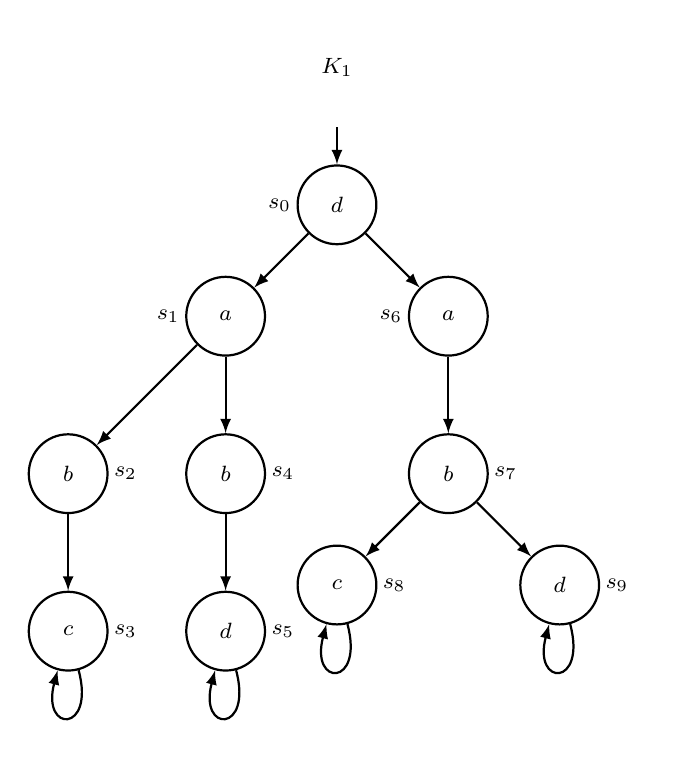
\begin{tikzpicture}[->,scale=1,label distance=-3mm,>= latex, node distance = 2cm]
    \tikzstyle{every node}=[shape=circle,minimum size=10mm,font=\footnotesize];
    \tikzstyle{every path} = [draw,thick];
    
    \node[draw] (n0) [label=left:$s_0$] {$d$};
    
    \node (tmp) [above of=n0, node distance=1.5cm] {};
    \node (tmp2) [above of=tmp,node distance=0.25cm] {$K_1$};
    
    \node[draw] (n6) [below right of=n0,label=left:$s_6$] {$a$};
    \node[draw] (n1) [below left of=n0,label=left:$s_1$] {$a$};
    \node[draw] (n4) [below of=n1,label=right:$s_4$] {$b$};
    \node[draw] (n2) [left of=n4,label=right:$s_2$] {$b$};
    \node[draw] (n3) [below of=n2,label=right:$s_3$] {$c$};
    \node[draw] (n5) [below of=n4,label=right:$s_5$] {$d$};
    \node[draw] (n8) [below of=n6,label=right:$s_7$] {$b$};
    \node[draw] (n9) [below left of=n8,label=right:$s_8$] {$c$};
    \node[draw] (n10) [below right of=n8,label=right:$s_{9}$] {$d$};
    
    \draw[->] (tmp) -- (n0);
    \draw[->] (n0) -- (n1);
    \draw[->] (n0) -- (n6);
    \draw[->] (n1) -- (n2);
    \draw[->] (n1) -- (n4);
    \draw[->] (n2) -- (n3);
    \draw[->] (n4) -- (n5);
		\draw[->] (n6) -- (n8);
		\draw[->] (n8) -- (n9);
		\draw[->] (n8) -- (n10);
		    
    \path[loop below] (n3) to (n3);
    \path[loop below] (n5) to (n5);
    \path[loop below] (n9) to (n9);
    \path[loop below] (n10) to (n10);
    
\end{tikzpicture}
}
\end{minipage}
\hfill
\begin{minipage}{0.48\textwidth}
	\scalebox{0.8}{
  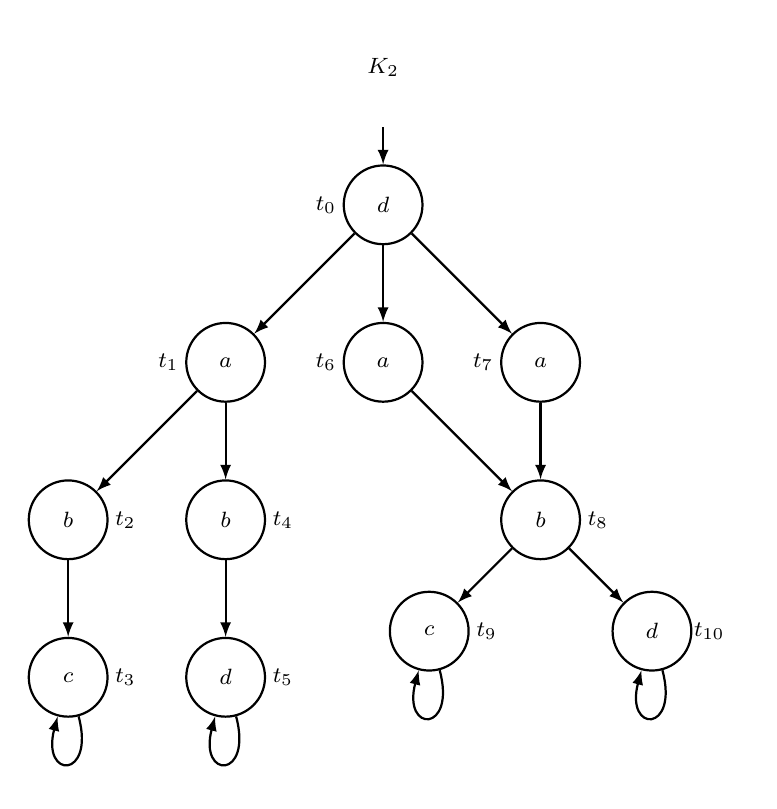
\begin{tikzpicture}[->,scale=1,label distance=-3mm,>= latex, node distance = 2cm]
    \tikzstyle{every node}=[shape=circle,minimum size=10mm,font=\footnotesize];
    \tikzstyle{every path} = [draw,thick];
    
    \node[draw] (n0) [label=left:$t_0$] {$d$};
    
    \node (tmp) [above of=n0, node distance=1.5cm] {};
    \node (tmp2) [above of=tmp,node distance=0.25cm] {$K_2$};
    
    \node[draw] (n6) [below of=n0,label=left:$t_6$] {$a$};
    \node[draw] (n1) [left of=n6,label=left:$t_1$] {$a$};
    \node[draw] (n7) [right of=n6,label=left:$t_7$] {$a$};
    \node[draw] (n4) [below of=n1,label=right:$t_4$] {$b$};
    \node[draw] (n2) [left of=n4,label=right:$t_2$] {$b$};
    \node[draw] (n3) [below of=n2,label=right:$t_3$] {$c$};
    \node[draw] (n5) [below of=n4,label=right:$t_5$] {$d$};
    \node[draw] (n8) [below of=n7,label=right:$t_8$] {$b$};
    \node[draw] (n9) [below left of=n8,label=right:$t_9$] {$c$};
    \node[draw] (n10) [below right of=n8,label=right:$t_{10}$] {$d$};
    
    \draw[->] (tmp) -- (n0);
    \draw[->] (n0) -- (n1);
    \draw[->] (n0) -- (n6);
    \draw[->] (n0) -- (n7);
    \draw[->] (n1) -- (n2);
    \draw[->] (n1) -- (n4);
    \draw[->] (n2) -- (n3);
    \draw[->] (n4) -- (n5);
		\draw[->] (n6) -- (n8);
		\draw[->] (n7) -- (n8);
		\draw[->] (n8) -- (n9);
		\draw[->] (n8) -- (n10);
		    
    \path[loop below] (n3) to (n3);
    \path[loop below] (n5) to (n5);
    \path[loop below] (n9) to (n9);
    \path[loop below] (n10) to (n10);
    
\end{tikzpicture}
}
\end{minipage}
\end{center}


\paragraph{a)} Give a simulation relation $H'$ such that $K_1 \leq K_2$ and $|H'| < |H|$.\hfill\textbf{(0.5 Points)}
\\

\textbf{Solution:}\\
\bigskip

To get the wanted simulation relation $H'$ you can remove either $(s_6,s_6)$ or $(s_6,s_7)$ from $H$.
We removed $(s_6,s_6)$ and got
$$H' = \{ (s_0, t_0), (s_1, t_1), (s_2, t_2), (s_3, t_3), (s_4, t_4), (s_5, t_5), $$
$$(s_6, t_7), (s_7, t_8), (s_8, t_9), (s_9, t_{10}) \}.$$

$|H'| = 10 < |H| = 11 \checkmark$

\paragraph{b)} Give a simulation relation $H''$ such that $K_1 \leq K_2$ and $|H''| > |H|$.\hfill\textbf{(0.5 Points)}
\\

\textbf{Solution:}\\
\bigskip

There are some possibilities, we've chosen this:\\
$$H'' = \{ (s_0, t_0), (s_1, t_1), (s_2, t_2), (s_3, t_3), (s_4, t_4), (s_5, t_5), $$
$$(s_6, t_6), (s_6, t_7), (s_7, t_8), (s_8, t_9), (s_9, t_{10}), (s_2,t_8), (s_4, t_8) \}.$$

$|H''| = 13 > |H| = 11 \checkmark$

\newpage
\Aufgabe[Simulation as refinement \hfill\textbf{(2 Points)}]
 
Given a \texttt{C} program and a set $AP$ of atomic propositions,
one can construct a Kripke structure over $AP$ which models the behaviour of the program with respect to the atomic propositions. 
For example, given the following program:

\begin{verbatim}
int x = 0, y = 0;
l0:
    for (int i = 0; i < 2; i++)
l1:     x = 1;
    y = *;
    if (y != 0)
l2:     x = 1;
    else
l3:     x = 0;
    goto l0;
\end{verbatim}

One may construct the following Kripke structure over $AP=\{x=0, y=0\}$
as follows:

\begin{center}
	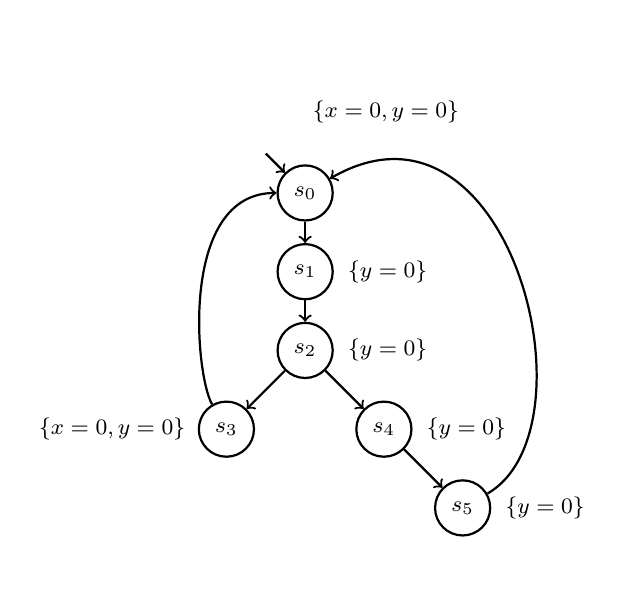
\begin{tikzpicture}[->,scale=1,label distance=0mm]
		\tikzstyle{every node}=[draw,shape=circle,minimum size=7mm,font=\footnotesize];
    \tikzstyle{every path}=[draw,thick];
    \node at (0, 0)   (s0) [label=above right:${ \{x=0,y=0\} }$]  {$s_0$};
    \node at (0, -1)  (s1) [label=right:${ \{y=0\} }$] {$s_1$};
    \node at (0, -2)  (s2) [label=right:${ \{y=0\} }$] {$s_2$};
    \node at (-1, -3) (s3) [label=left:${ \{x=0,y=0\} }$] {$s_3$};
    \node at (1, -3)  (s4) [label=right:${ \{y=0\} }$] {$s_4$};
    \node at (2, -4)  (s5) [label=right:${ \{y=0\} }$] {$s_5$};

    \draw (-0.5, 0.5) to (s0);
    \draw (s0) to (s1);
    \draw (s1) to (s2);
    \draw (s2) to (s3);
    \draw (s2) to (s4);
    \draw (s3) .. controls +(120:8mm) and +(left:16mm) .. (s0);
    \draw (s4) to (s5);
    \draw (s5) .. controls +(30:20mm) and +(30:30mm) .. (s0);
	\end{tikzpicture}
\end{center}
In the example above, the special
form of assignment \texttt{y = *} denotes a non-deterministic assignment
to~\texttt{y} of any value from the domain of \texttt{y}, e.g., it can be
assigned concurrently by another thread.
The effect of a statement sequence residing under the same label $\ell_j$ may
be merged into one state, whereas the effect of statements marked with
distinct labels $\ell_j$ and $\ell_k$, $j \ne k$, must not be merged into one
state.

\paragraph{a)}
Construct a Kripke structure $K$ over
$AP=\{port\_o=0,port\_o=1,port\_o=2,port\_o=3\}$ for the following program:

\begin{verbatim}
int locked_dev = 0, port_o = 0, port_i = 0;
l0:
    for (int i = 0; i < 3; i++)
l1:     port_o = 1;

    port_i = *;
    if (port_i < 3) {
        goto l0;
    }
    do {
l2:     port_o = 2; locked_dev = *;
    } while (locked_dev);
l3: locked_dev = 1; port_i = *;
    if (port_i == 1)
l4:     port_o = 1;
    else
l5:     port_o = 3;
l6: port_o = 0; locked_dev = 0;
    goto l0;
\end{verbatim}


\paragraph{b)}
Give simulation relations between $K$ and the following Kripke structures
 $S'$ (left) and $S''$ (right):

\begin{center}
	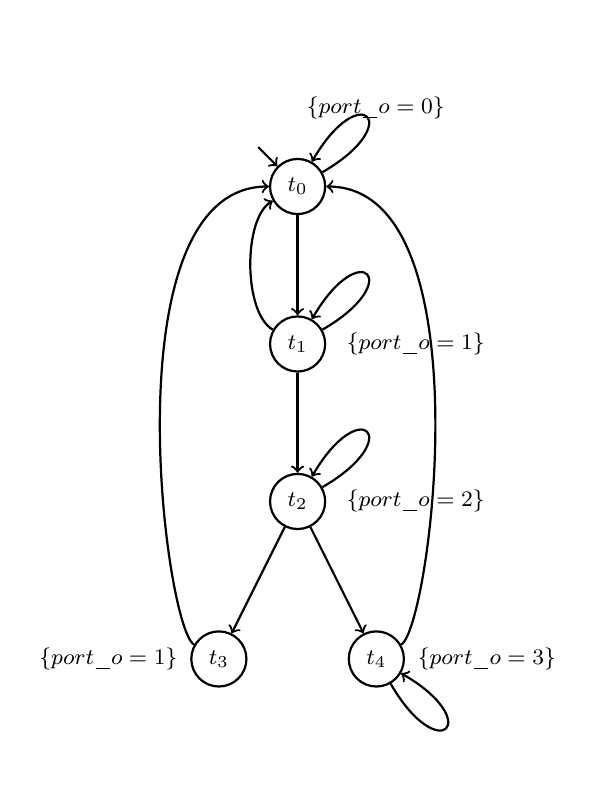
\begin{tikzpicture}[->,scale=1,label distance=0mm]
		\tikzstyle{every node}=[draw,shape=circle,minimum size=7mm,font=\footnotesize];
    \tikzstyle{every path}=[draw,thick];
    \node at (0, 0)   (s0) [label=above right:${ \{port\_o=0\} }$]  {$t_0$};
    \node at (0, -2)  (s1) [label=right:${ \ \{port\_o=1\} }$] {$t_1$};
    \node at (0, -4)  (s2) [label=right:${ \ \{port\_o=2\} }$] {$t_2$};
    \node at (-1, -6) (s3) [label=left:${ \{port\_o=1\} }$] {$t_3$};
    \node at (1, -6)  (s4) [label=right:${ \{port\_o=3\} }$] {$t_4$};

    \draw (-0.5, 0.5) to (s0);
    \draw (s0) to (s1);
    \draw (s0)  .. controls +(30:16mm) and +(60:16mm) .. (s0);
    \draw (s1)  .. controls +(150:8mm) and +(210:8mm) .. (s0);
    \draw (s1)  .. controls +(30:16mm) and +(60:16mm) .. (s1);
    \draw (s1) to (s2);
    \draw (s2)  .. controls +(30:16mm) and +(60:16mm) .. (s2);
    \draw (s2) to (s3);
    \draw (s2) to (s4);
    \draw (s3) .. controls +(150:8mm) and +(left:24mm) .. (s0);
    \draw (s4) .. controls +(30:8mm) and +(right:24mm) .. (s0);
    \draw (s4)  .. controls +(300:16mm) and +(330:16mm) .. (s4);
    	\end{tikzpicture}
	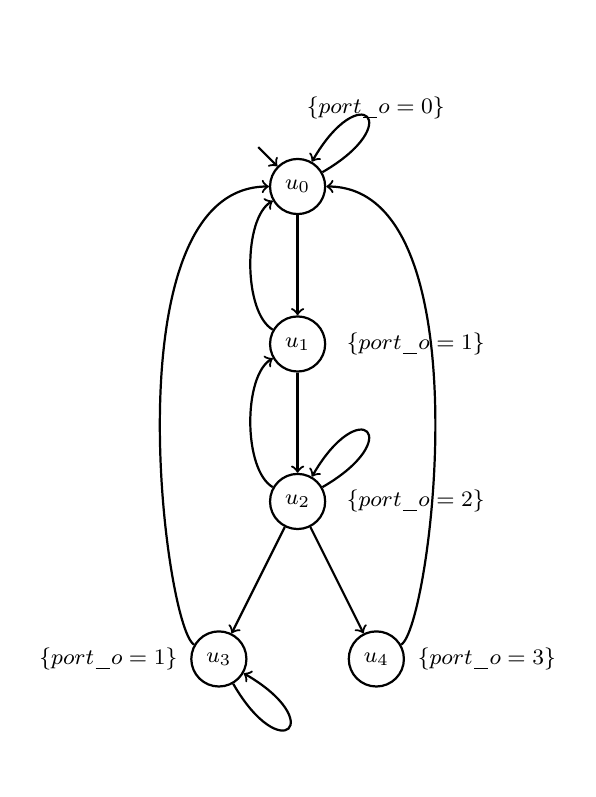
\begin{tikzpicture}[->,scale=1,label distance=0mm]
		\tikzstyle{every node}=[draw,shape=circle,minimum size=7mm,font=\footnotesize];
    \tikzstyle{every path}=[draw,thick];
    \node at (0, 0)   (s0) [label=above right:${ \{port\_o=0\} }$]  {$u_0$};
    \node at (0, -2)  (s1) [label=right:${ \ \{port\_o=1\} }$] {$u_1$};
    \node at (0, -4)  (s2) [label=right:${ \ \{port\_o=2\} }$] {$u_2$};
    \node at (-1, -6) (s3) [label=left:${ \{port\_o=1\} }$] {$u_3$};
    \node at (1, -6)  (s4) [label=right:${ \{port\_o=3\} }$] {$u_4$};

    \draw (-0.5, 0.5) to (s0);
    \draw (s0) to (s1);
    \draw (s0)  .. controls +(30:16mm) and +(60:16mm) .. (s0);
    \draw (s1)  .. controls +(150:8mm) and +(210:8mm) .. (s0);
    \draw (s2)  .. controls +(150:8mm) and +(210:8mm) .. (s1);
    \draw (s1) to (s2);
    \draw (s2)  .. controls +(30:16mm) and +(60:16mm) .. (s2);
    \draw (s2) to (s3);
    \draw (s2) to (s4);
    \draw (s3) .. controls +(150:8mm) and +(left:24mm) .. (s0);
    \draw (s3) .. controls +(300:16mm) and +(330:16mm) .. (s3);
    \draw (s4) .. controls +(30:8mm) and +(right:24mm) .. (s0);
    	\end{tikzpicture}
\end{center}

$\ddot\smile$ \textbf{Solution}\\
\begin{enumerate}
\item
Kripke structure $K$:
\begin{center}
	\begin{tikzpicture}[->,scale=1,label distance=0mm]
		\tikzstyle{every node}=[draw,shape=circle,minimum size=7mm,font=\footnotesize];
    \tikzstyle{every path}=[draw,thick];
    \node at (0, 0)   (s0) [label=right:${ \{port\_o=0\} }$]  {$s_0$};
    \node at (0, -2)  (s1) [label=upper right:${ \ \{port\_o=1\} }$] {$s_1$};
    \node at (0, -4)  (s2) [label=right:${ \ \{port\_o=1\} }$] {$s_2$};
    \node at (0, -6)  (s3) [label=bottom right:${ \ \{port\_o=1\} }$] {$s_3$};
    \node at (-1, -8) (s4) [label=left:${ \{port\_o=1\} }$] {$s_4$};
    \node at (1, -8)  (s5) [label=right:${ \{port\_o=2\} }$] {$s_5$};
    \node at (0, -10) (s6) [label=left:${ \{port\_o=1\} }$] {$s_6$};
    \node at (2, -10)  (s7) [label=right:${ \{port\_o=3\} }$] {$s_7$};
    \node at (1, -12)  (s8) [label=upper:${ \ \{port\_o=0\} }$] {$s_8$};

    \draw (-0.5, 0.5) to (s0);
    \draw (s0) to (s1);
    \draw (s1) to (s2);
    \draw (s2) to (s3);
    \draw (s3) to (s4);
    \draw (s3) to (s5);
    \draw (s4) .. controls +(150:8mm) and +(left:24mm) .. (s1);
    \draw (s5) .. controls +(30:16mm) and +(60:16mm) .. (s5);
    \draw (s5) to (s6);
    \draw (s5) to (s7);
    \draw (s6) to (s8);
    \draw (s7) to (s8);
    \draw (s8)  .. controls +(20:170mm) and +(20:60mm) .. (s0);
    	\end{tikzpicture}
\end{center}

\item
$S'$ simulates $K$ with the following simulation relation\\
$$H' = \{(s_0,t_0),(s_1,t_1),(s_2,t_1),(s_3,t_1),(s_4,t_1),(s_5,t_2),(s_6,t_3),(s_7,t_4),(s_8,t_0)\}.$$
ans $S''$ simulates $K$ with the following simulation relation\\
$$H'' = \{(s_0,u_0),(s_1,u_3),(s_2,u_3),(s_3,u_1),(s_4,u_3),(s_5,u_2),(s_6,u_3),(s_7,u_4),(s_8,u_0)\}.$$
$K$ doesn't simulate neither $S'$ nor $S''$, because there doesn't exist any state with AP $\{port\_o=0\}$ which has a path to $\{port\_o=0\}$ and $\{port\_o=1\}$...
\end{enumerate}

\newpage
\Aufgabe[Predicate Abstraction\hfill\textbf{(1.5 Point)}]
Consider the following program:
\begin{verbatim}
void foo(int j, int z) {
  assume(z != 0);
  int i := j;
  while(z != 0) {
      i := i + z;
      if(z > 0)
          z--
      else
          z ++;
  };
  assert(i != j)
}
\end{verbatim}

The {\em assume statement} at the beginning of the function forces the parameter $z$ not to be 0 when the function is called.

\begin{enumerate}

 \item Argue in your own words why the assertion at the end of the program allways holds, i.e., why the error state can never be reached.

 \item Provide a labeled transition system for the given program.

 \item Provide an abstraction for the labeled transition system that uses the predicates $i = j$, $i < j$, $i > j$.

 \item Check whether the error state can be reached in the abstraction, if so state a trace to the error state and refine the abstraction with suitable predicates such that the error state is not reachable anymore.

\end{enumerate}


\textbf{Solution:}\\
\medskip
\begin{enumerate}
\item The call of the method \texttt{\small assume(z != 0)} in the beginning
of the program forces, that the value of the variable $z$ is not $0$. Since
the semantics of \texttt{\small assume(x)}, means that "by assumption \texttt%
{\small x} holds" and by definition an assumption can never being violated.
Thus, the while-loop will be executed at least one time, regardless if the
value of $z$ is positive or negative.

Since the if-condition inside of the loop controls $z$ by decrementing or
incrementing and consequently the variable $i$ will also incremented or
decremented. Thus, the loop will be executed exactly in $|z|$ times. Since  $%
i=j$ is in the precondition of the loop, the loop is guaranteed to terminate
since $z\neq 0$. Hence, after the termination of the while-loop, the case
that $i=j$ will never reached, i.e. it will never hold.
\newpage

\item \textit{Labeled Transiton System (LTS):}

\begin{figure}[th]
\centering
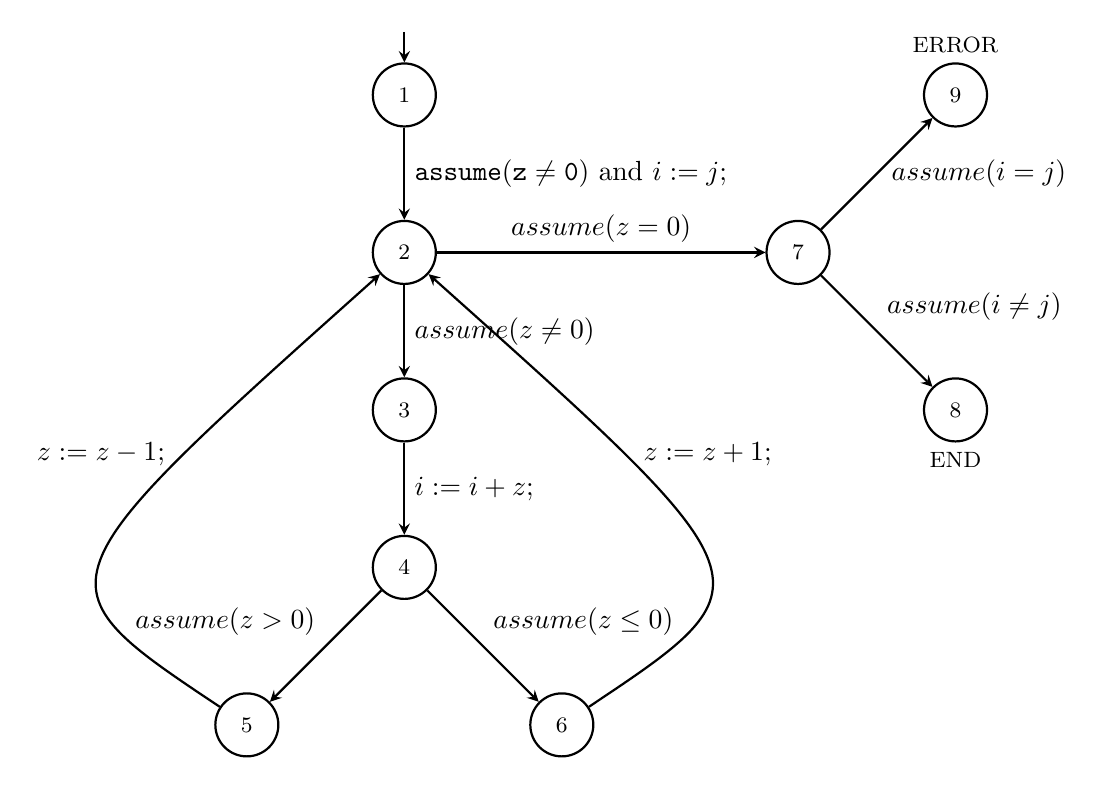
\begin{tikzpicture}[->, >=stealth, line join=bevel]
	\pgfsetlinewidth{1bp}
	\pgfsetcolor{black}

	\tikzstyle{state} = [draw,shape=circle,minimum size=8mm,font=\footnotesize];
	\tikzstyle{accept_state} = [shape=circle, minimum size=8mm, accepting, font=\small, draw];
	\tikzstyle{every path} = [draw, thick];

	\node[state] at (0,10) (1) {$1$};
	\node[state] at (0,8) (2) {$2$}; 
	\node[state] at (0,6) (3) {$3$}; 
	\node[state] at (0,4) (4) {$4$}; 
	\node[state] at (-2,2) (5) {$5$}; 
	\node[state] at (2,2) (6) {$6$}; 
	\node[state] at (5,8) (7) {$7$}; 
	\node[state] at (7,6) (8) [label=below:{\footnotesize END}] {$8$}; 
	\node[state] at (7,10) (9) [label=above:{\footnotesize ERROR}] {$9$}; 

	\draw (0, 10.8) to (1);
	\draw (1) to node[auto] {$\mbox{\fontsize{10}{11}\selectfont $\mathtt{assume(z \neq 0)} \mbox{ and } i := j;$}$} (2);
	\draw (2) to node[auto] {$\mbox{\fontsize{10}{11}\selectfont $assume(z \neq 0)$}$} (3);
	\draw (3) to node[auto] {$\mbox{\fontsize{10}{11}\selectfont $i := i+z;$}$} (4);
	\draw (4) to node[auto, swap] {$\mbox{\fontsize{10}{11}\selectfont $assume(z > 0)$}$} (5);
	\draw (4) to node[auto] {$\mbox{\fontsize{10}{11}\selectfont $assume(z \leq 0)$}$} (6);
	\draw (2) to node[auto] {$\mbox{\fontsize{10}{11}\selectfont $assume(z = 0)$}$} (7);
	\draw (7) to node[auto] {$\mbox{\fontsize{10}{11}\selectfont $assume(i \neq j)$}$} (8);
	\draw (7) to node[right] {$\mbox{\fontsize{10}{11}\selectfont $\,assume(i = j)$}$} (9);
	\draw[->] (5) .. controls (-4.7,3.8) .. (2) node[pos=.75, left] {$z := z-1;\;$};
	\draw[->] (6) .. controls (4.7,3.8) .. (2) node[pos=.75, right] {$\;z := z+1;$};
\end{tikzpicture}
\caption{{\protect\small LTS of the given program.}}
\label{lts_program}
\end{figure}

\item The corresponding predicates for the abstract transition system $%
TS^{abstract}$ (see figure \ref{abstraction_graph}) are defined as follows:%
\begin{equation*}
e\equiv i=j,\quad l\equiv i<j\quad \text{and\quad }g\equiv i>j,
\end{equation*}

where $e$ denotes the case that $(i=j)$ holds and $\overline{e}$ denotes the
that case $(i=j)$ does not hold in the current state. This definition holds
also for the predicates $l$ and $g$.

A possible error trail would be for example $(1,l\overline{g}\overline{e}%
)\rightarrow (2,\overline{l}\overline{g}e)\rightarrow (7,\overline{l}%
\overline{g}e)\rightarrow (9,\overline{l}\overline{g}e)$. Since by the
definition of assumption, an assumption can be never violated, the
error state $(9,\overline{l}\overline{g}e)$ in $TS^{abstract}$ will never
reached.

\begin{figure}[th]
\centering
% Start of code
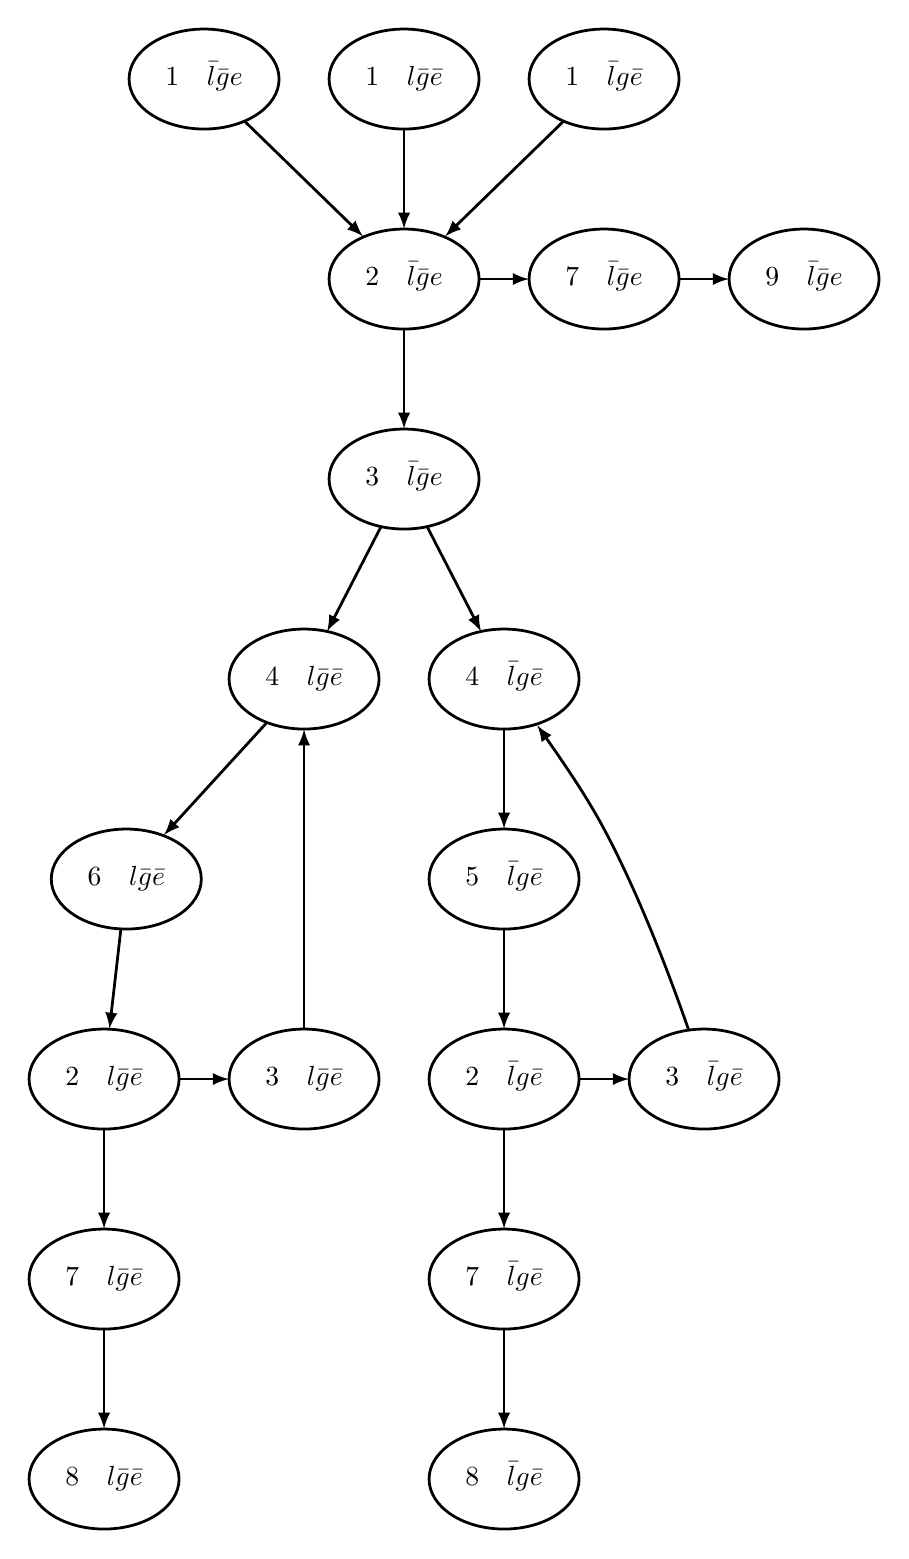
\begin{tikzpicture}[anchor=mid,>=latex,line join=bevel]
%\begin{tikzpicture}[>=latex,line join=bevel]
  \pgfsetlinewidth{1bp}
%%
\pgfsetcolor{black}
  % Edge: 15 -> 17
  \draw [->] (171bp,71.697bp) .. controls (171bp,63.983bp) and (171bp,54.712bp)  .. (171bp,36.104bp);
  % Edge: 5 -> 6
  \draw [->] (126.65bp,360.76bp) .. controls (122.29bp,352.28bp) and (116.85bp,341.71bp)  .. (107.3bp,323.15bp);
  % Edge: 10 -> 12
  \draw [->] (54bp,162bp) .. controls (56.615bp,162bp) and (59.229bp,162bp)  .. (71.93bp,162bp);
  % Edge: 5 -> 7
  \draw [->] (143.35bp,360.76bp) .. controls (147.71bp,352.28bp) and (153.15bp,341.71bp)  .. (162.7bp,323.15bp);
  % Edge: 4 -> 18
  \draw [->] (162bp,450bp) .. controls (164.61bp,450bp) and (167.23bp,450bp)  .. (179.93bp,450bp);
  % Edge: 12 -> 6
  \draw [->] (99bp,180.19bp) .. controls (99bp,204.42bp) and (99bp,248.89bp)  .. (99bp,287.87bp);
  % Edge: 18 -> 19
  \draw [->] (234bp,450bp) .. controls (236.61bp,450bp) and (239.23bp,450bp)  .. (251.93bp,450bp);
  % Edge: 14 -> 16
  \draw [->] (27bp,71.697bp) .. controls (27bp,63.983bp) and (27bp,54.712bp)  .. (27bp,36.104bp);
  % Edge: 4 -> 5
  \draw [->] (135bp,431.7bp) .. controls (135bp,423.98bp) and (135bp,414.71bp)  .. (135bp,396.1bp);
  % Edge: 11 -> 13
  \draw [->] (198bp,162bp) .. controls (200.61bp,162bp) and (203.23bp,162bp)  .. (215.93bp,162bp);
  % Edge: 10 -> 14
  \draw [->] (27bp,143.7bp) .. controls (27bp,135.98bp) and (27bp,126.71bp)  .. (27bp,108.1bp);
  % Edge: 13 -> 7
  \draw [->] (237.38bp,179.88bp) .. controls (231.03bp,198.14bp) and (219.88bp,227.89bp)  .. (207bp,252bp) .. controls (201.73bp,261.86bp) and (195.05bp,272.15bp)  .. (182.95bp,289.32bp);
  % Edge: 1 -> 4
  \draw [->] (77.57bp,506.83bp) .. controls (87.75bp,496.94bp) and (101.52bp,483.55bp)  .. (120.2bp,465.38bp);
  % Edge: 8 -> 10
  \draw [->] (33.022bp,215.7bp) .. controls (32.141bp,207.98bp) and (31.081bp,198.71bp)  .. (28.955bp,180.1bp);
  % Edge: 7 -> 9
  \draw [->] (171bp,287.7bp) .. controls (171bp,279.98bp) and (171bp,270.71bp)  .. (171bp,252.1bp);
  % Edge: 11 -> 15
  \draw [->] (171bp,143.7bp) .. controls (171bp,135.98bp) and (171bp,126.71bp)  .. (171bp,108.1bp);
  % Edge: 3 -> 4
  \draw [->] (192.43bp,506.83bp) .. controls (182.25bp,496.94bp) and (168.48bp,483.55bp)  .. (149.8bp,465.38bp);
  % Edge: 6 -> 8
  \draw [->] (85.427bp,290.15bp) .. controls (76.688bp,280.6bp) and (65.166bp,267.99bp)  .. (48.553bp,249.82bp);
  % Edge: 9 -> 11
  \draw [->] (171bp,215.7bp) .. controls (171bp,207.98bp) and (171bp,198.71bp)  .. (171bp,180.1bp);
  % Edge: 2 -> 4
  \draw [->] (135bp,503.7bp) .. controls (135bp,495.98bp) and (135bp,486.71bp)  .. (135bp,468.1bp);
  % Node: 11
\begin{scope}
  \definecolor{strokecol}{rgb}{0.0,0.0,0.0};
  \pgfsetstrokecolor{strokecol}
  \draw (171bp,162bp) ellipse (27bp and 18bp);
  \draw (171bp,162bp) node {$2 \quad \bar{l}g\bar{e}$};
\end{scope}
  % Node: 10
\begin{scope}
  \definecolor{strokecol}{rgb}{0.0,0.0,0.0};
  \pgfsetstrokecolor{strokecol}
  \draw (27bp,162bp) ellipse (27bp and 18bp);
  \draw (27bp,162bp) node {$2 \quad l\bar{g}\bar{e}$};
\end{scope}
  % Node: 13
\begin{scope}
  \definecolor{strokecol}{rgb}{0.0,0.0,0.0};
  \pgfsetstrokecolor{strokecol}
  \draw (243bp,162bp) ellipse (27bp and 18bp);
  \draw (243bp,162bp) node {$3 \quad \bar{l}g\bar{e}$};
\end{scope}
  % Node: 12
\begin{scope}
  \definecolor{strokecol}{rgb}{0.0,0.0,0.0};
  \pgfsetstrokecolor{strokecol}
  \draw (99bp,162bp) ellipse (27bp and 18bp);
  \draw (99bp,162bp) node {$3 \quad l\bar{g}\bar{e}$};
\end{scope}
  % Node: 15
\begin{scope}
  \definecolor{strokecol}{rgb}{0.0,0.0,0.0};
  \pgfsetstrokecolor{strokecol}
  \draw (171bp,90bp) ellipse (27bp and 18bp);
  \draw (171bp,90bp) node {$7 \quad \bar{l}g\bar{e}$};
\end{scope}
  % Node: 14
\begin{scope}
  \definecolor{strokecol}{rgb}{0.0,0.0,0.0};
  \pgfsetstrokecolor{strokecol}
  \draw (27bp,90bp) ellipse (27bp and 18bp);
  \draw (27bp,90bp) node {$7 \quad l\bar{g}\bar{e}$};
\end{scope}
  % Node: 17
\begin{scope}
  \definecolor{strokecol}{rgb}{0.0,0.0,0.0};
  \pgfsetstrokecolor{strokecol}
  \draw (171bp,18bp) ellipse (27bp and 18bp);
  \draw (171bp,18bp) node {$8 \quad \bar{l}g\bar{e}$};
\end{scope}
  % Node: 16
\begin{scope}
  \definecolor{strokecol}{rgb}{0.0,0.0,0.0};
  \pgfsetstrokecolor{strokecol}
  \draw (27bp,18bp) ellipse (27bp and 18bp);
  \draw (27bp,18bp) node {$8 \quad l\bar{g}\bar{e}$};
\end{scope}
  % Node: 19
\begin{scope}
  \definecolor{strokecol}{rgb}{0.0,0.0,0.0};
  \pgfsetstrokecolor{strokecol}
  \draw (279bp,450bp) ellipse (27bp and 18bp);
  \draw (279bp,450bp) node {$9 \quad \bar{l}\bar{g}e$};
\end{scope}
  % Node: 18
\begin{scope}
  \definecolor{strokecol}{rgb}{0.0,0.0,0.0};
  \pgfsetstrokecolor{strokecol}
  \draw (207bp,450bp) ellipse (27bp and 18bp);
  \draw (207bp,450bp) node {$7 \quad \bar{l}\bar{g}e$};
\end{scope}
  % Node: 1
\begin{scope}
  \definecolor{strokecol}{rgb}{0.0,0.0,0.0};
  \pgfsetstrokecolor{strokecol}
  \draw (63bp,522bp) ellipse (27bp and 18bp);
  \draw (63bp,522bp) node {$1 \quad \bar{l}\bar{g}e$};
\end{scope}
  % Node: 3
\begin{scope}
  \definecolor{strokecol}{rgb}{0.0,0.0,0.0};
  \pgfsetstrokecolor{strokecol}
  \draw (207bp,522bp) ellipse (27bp and 18bp);
  \draw (207bp,522bp) node {$1 \quad \bar{l}g\bar{e}$};
\end{scope}
  % Node: 2
\begin{scope}
  \definecolor{strokecol}{rgb}{0.0,0.0,0.0};
  \pgfsetstrokecolor{strokecol}
  \draw (135bp,522bp) ellipse (27bp and 18bp);
  \draw (135bp,522bp) node {$1 \quad l\bar{g}\bar{e}$};
\end{scope}
  % Node: 5
\begin{scope}
  \definecolor{strokecol}{rgb}{0.0,0.0,0.0};
  \pgfsetstrokecolor{strokecol}
  \draw (135bp,378bp) ellipse (27bp and 18bp);
  \draw (135bp,378bp) node {$3 \quad \bar{l}\bar{g}e$};
\end{scope}
  % Node: 4
\begin{scope}
  \definecolor{strokecol}{rgb}{0.0,0.0,0.0};
  \pgfsetstrokecolor{strokecol}
  \draw (135bp,450bp) ellipse (27bp and 18bp);
  \draw (135bp,450bp) node {$2 \quad \bar{l}\bar{g}e$};
\end{scope}
  % Node: 7
\begin{scope}
  \definecolor{strokecol}{rgb}{0.0,0.0,0.0};
  \pgfsetstrokecolor{strokecol}
  \draw (171bp,306bp) ellipse (27bp and 18bp);
  \draw (171bp,306bp) node {$4 \quad \bar{l}g\bar{e}$};
\end{scope}
  % Node: 6
\begin{scope}
  \definecolor{strokecol}{rgb}{0.0,0.0,0.0};
  \pgfsetstrokecolor{strokecol}
  \draw (99bp,306bp) ellipse (27bp and 18bp);
  \draw (99bp,306bp) node {$4 \quad l\bar{g}\bar{e}$};
\end{scope}
  % Node: 9
\begin{scope}
  \definecolor{strokecol}{rgb}{0.0,0.0,0.0};
  \pgfsetstrokecolor{strokecol}
  \draw (171bp,234bp) ellipse (27bp and 18bp);
  \draw (171bp,234bp) node {$5 \quad \bar{l}g\bar{e}$};
\end{scope}
  % Node: 8
\begin{scope}
  \definecolor{strokecol}{rgb}{0.0,0.0,0.0};
  \pgfsetstrokecolor{strokecol}
  \draw (35bp,234bp) ellipse (27bp and 18bp);
  \draw (35bp,234bp) node {$6 \quad l\bar{g}\bar{e}$};
\end{scope}
%
\end{tikzpicture}
% End of code
\caption{{\protect\small The abstract transition system $TS^{abstract}$ of the above LTS (\ref{lts_program}), where the state $8$ denotes the final \textit{terminal state} and state $9$ the \textit{error state}.}}
\label{abstraction_graph}
\end{figure}

\item By adding a new predicate symbol $z$ to the set of predicates $P=\{l,g,e\}$
of the abstract transition system $TS^{abstract}$, we achieve a new abstract
transition system. The new predicate $z$ denotes the case that $(z\neq 0)$
holds, whereas $\overline{z}$ denotes that $(z\neq 0)$ does not hold in the
current state. Then the resulting abstract transition system is the same as
shown in \textit{c.)}, but without the path to the error state, since the
states $(7,\overline{l}\overline{g}e)$ and $(9,\overline{l}\overline{g}e)$
will never reached.


\end{enumerate}
\newpage
%%%%%%%%%%%%%%%%%%%%%%%%%%%%%%%%%%%%%%%%%%%%%%%%%%%%%%%%%%%%%%%%%%%%%%
%% Aufgabe
\Aufgabe[Bounded Model Checking\hfill\textbf{(1.5 Point)}]
Consider the following Program:

\lstinputlisting[basicstyle=\footnotesize]{main.c}

The Matrix $G$ models a graph with $N$ nodes, i.e, $G[i][j]$ is true iff there is a directed edge from node $i$ to node $j$. The method $\mathit{nondet}$ chooses an integer non-deterministically.

\begin{enumerate}
	\item Use CBMC to find the lowest value for $K$ such that the assertion at the end of the program can be violated. What does it mean that the error state is or is not reachable for a given graph $G$ and a given value $K$?

	\item Perform an unwinding of the loop for $K = 3$.
				
	\item Transform the unwinded program into the SSA form.
	
	\item Build a semantically equivalent SMT formula from the SSA form. {\em Note:} A call to $\mathit{nondet}$ can be modeled by introducing a new integer variable.

        \item Can you draw a conclusion about the satisfiability of the formula by comparing the value for $K$ that you determined under $(a)$ with the number of times the loop was unwinded for building the formula? Check whether the formula can be satisfied (You may use an SMT solver such as {\em Yices} or {\em Z3}) to be sure that the result of the satisfiability check is consistent with your expectation.

\end{enumerate}

\vspace{0.5cm}
\\

$\ddot\smile$ \textbf{Solution}\\
\begin{enumerate}
\item
The lowest value $K$ for a violated assertion is $1$.

\item[(b) \& (c)] \quad
\medskip
\begin{lstlisting}[	frame=lines, mathescape=true,
					caption={ Unwinded code in SSA form:},
					label={unw_func}]
void main() {
	// Intialization:
	bool G[N][N] = {{$\ldots$}};
	bool result$_0$ = 1;
	int node$_0$ = 0;
	int next$_0$ = 0;
	int i$_0$ = 0;
	
	// Unwinding of the for-loop for $K = 3$:
	// First iteration:
	if(i$_0$ < K) {
		next$_1$ = nondet();
		result$_1$ = result$_0$ && G[node$_0$][next$_1$];
		node$_1$ = next$_1$;
		i$_1$ = i$_0$ + 1;
	// Second iteration:
		if(i$_1$ < K) {
			next$_2$ = nondet();
			result$_2$ = result$_1$ && G[node$_1$][next$_2$];
			node$_2$ = next$_2$;
			i$_2$ = i$_1$ + 1;
		// Third iteration + termination:
			if(i$_2$ < K) {
				next$_3$ = nondet();
				result$_3$ = result$_2$ && G[node$_2$][next$_3$];
				node$_3$ = next$_3$;
				i$_3$ = i$_2$ + 1;
				assert(!(i$_3$ < K));
			}
		}
	}
	result$_4$ = result$_3$ && node$_3$ == 0);
	assert(!result$_4$);
}
\end{lstlisting}

\item[(d)]
\item[(e)]
\end{enumerate}
\newpage
\Aufgabe[Computing the (Greatest) Bisimulation Relation \hfill\textbf{(1 Point)}]

Let $K_1 = (S_1, R_1, L_1)$ and  $K_2 = (S_2, R_2, L_2)$ be two Kripke structures over a set of atomic predicates $\mathit{AP}$.
The relations $H_n \subseteq S_1 \times S_2$ are inductively defined by:
\begin{itemize}
\item $(s_1,s_2) \in H_0$ iff $L_1(s_1) = L_2(s_2)$.
\item $(s_1,s_2) \in H_{n+1}$ iff
    \begin{enumerate}[(i)]
    \item $(s_1,s_2) \in H_n$,\qquad ($\star$)
    \item for all $(s_1,t_1) \in R_1$ there exists a $(s_2,t_2) \in R_2$ with $(t_1,t_2) \in H_n$, and
    \item for all $(s_2,t_2) \in R_2$ there exists a $(s_1,t_1) \in R_1$ with $(t_1,t_2) \in H_n$.
    \end{enumerate}
\end{itemize}

\begin{enumerate}

	\item Compute the sequence $H_0, H_1, H_2,\ldots$ for the Kripke structures $K_1$ and $K_2$ from Exercise 2.
    
	\item Show that the sequence $H_0, H_1, H_2,\ldots$ \emph{stabilizes} for all finite Kripke structures $K_1$ and $K_2$, i.e., there is a $n \ge 0$ such that $H_n = H_{n+1}$.
    
	\item Construct Kripke structures $K_1^n$ and $K_2^n$ such that the sequence $H_0, H_1, H_2,\ldots$ stabilizes after exactly $n$ steps.

\end{enumerate}

a.)

\textbf{Solution:}

\bigskip

Let $K_{1}=(S,R,L_{1})$ and $K_{2}=(S,R,L_{2})$ be two Kripke structures
with the same set of states $S$ and the same transition relation $R$ such
that $L_{1}(s)\subseteq L_{2}(s),\Forall s\in S$.\medskip

Let $H^{\ast }$ be the \textit{largest possible bisimulation} between the
structures $K_{1}$ and $K_{2}$ with $S=S_{1}=S_{2}$ and $R=R_{1}=R_{2}$.

Since both structures $K_{1}$ and $K_{2}$ are finite, then the above
inductive definition for relations $H_{n}\subseteq S_{1}\times S_{2}$
(procedure) is guaranteed to terminate.

Let $H^{\ast }:=\bigcap\nolimits_{i}H_{i}$, and%
\begin{equation*}
(s_{1},s_{2})\in H^{\ast }\quad \text{iff\quad }(s_{1},s_{2})\in H_{i}\text{
for all }i\geq 0.
\end{equation*}

Then by definition, $H_{i}\supseteq H_{i+1}$ for all $i\geq 0$. Thus $%
H^{\ast }$ can be computed by a fixed point iteration as follows:%
\begin{eqnarray*}
&&H_{0}=\{(s_{1},s_{2})\in S_{1}\times S_{2}\mid L_{1}(s_{1})\subseteq
L_{2}(s_{2})\} \\
&&H_{1}=\{(s_{1},s_{2})\in S_{1}\times S_{2}\mid (s_{1},s_{2})\in H_{1} \AND%
\Forall (s_{1},t_{1})\in R_{1}\IMPL\Exists (s_{2},t_{2})\in R_{2}\text{ s.t. }%
(t_{1},t_{2})\in H_{1}\AND \\
&&\Forall (s_{2},t_{2})\in R_{2}\IMPL\Exists (s_{1},t_{1})\in R_{1}\text{
s.t. }(t_{1},t_{2})\in H_{1}\} \\
&&H_{2}=\{(s_{1},s_{2})\in S_{1}\times S_{2}\mid (s_{1},s_{2})\in H_{2}\AND%
\Forall(s_{1},t_{1})\in R_{1}\IMPL\Exists (s_{2},t_{2})\in R_{2}\text{ s.t. }%
(t_{1},t_{2})\in H_{2}\AND \\
&&\Forall (s_{2},t_{2})\in R_{2}\IMPL\Exists (s_{1},t_{1})\in R_{1}\text{
s.t. }(t_{1},t_{2})\in H_{2}\} \\
&&\ldots \\
&&H_{i}=\{(s_{1},s_{2})\in S_{1}\times S_{2}\mid (s_{1},s_{2})\in H_{i} \AND%
\Forall (s_{1},t_{1})\in R_{1}\IMPL\Exists (s_{2},t_{2})\in R_{2}\text{ s.t. }%
(t_{1},t_{2})\in H_{i}\AND \\
&&\Forall (s_{2},t_{2})\in R_{2}\IMPL\Exists (s_{1},t_{1})\in R_{1}\text{
s.t. }(t_{1},t_{2})\in H_{i}\} \\
&&H_{i+1}=\{(s_{1},s_{2})\in S_{1}\times S_{2}\mid (s_{1},s_{2})\in H_{i+1}%
\AND\Forall (s_{1},t_{1})\in R_{1}\IMPL\Exists (s_{2},t_{2})\in R_{2}\text{
s.t. }(t_{1},t_{2})\in H_{i+1}\AND \\
&&\Forall (s_{2},t_{2})\in R_{2}\IMPL\Exists (s_{1},t_{1})\in R_{1}\text{
s.t. }(t_{1},t_{2})\in H_{i+1}\}\quad \text{(successor stage)} \\
&&\ldots \\
&&H_{n}=\{(s_{1},s_{2})\in S_{1}\times S_{2}\mid (s_{1},s_{2})\in H_{n} \AND%
\Forall (s_{1},t_{1})\in R_{1}\IMPL\Exists (s_{2},t_{2})\in R_{2}\text{ s.t. }%
(t_{1},t_{2})\in H_{n}\AND \\
&&\Forall(s_{2},t_{2})\in R_{2}\IMPL\Exists (s_{1},t_{1})\in R_{1}\text{
s.t. }(t_{1},t_{2})\in H_{n}\} \\
&&H_{n+1}=H_{n}\quad \text{i.e. }H_{n}=\tbigcap\nolimits_{i<n}H_{i}\quad\text{%
(limit stage).}
\end{eqnarray*}

Since $K_{1}$ and $K_{2}$ are finite, then $\Exists n\in \mathbb{N}$ such
that $H_{n}=H_{n+1}$. Therefore, it is easy to see that $H_{n}$ is exactly $%
H^{\ast }$. Moreover, two Kripke structures $K_{1}$ and $K_{2}$ are $H^{\ast
}$-equivalent if for every initial state $s_{0}\in S_{1}$ in $K_{1}$ there
is also an initial state $s_{1}\in S_{2}$ in $K_{2}$ such that $%
(s_{0},s_{1})\in H^{\ast }$.

\bigskip 

b.)

\textbf{Solution:}

\medskip

We show that $H^{\ast }$ is indeed the largest bisimulation between $K_{1}$
and $K_{2}$. This means, that every bisimulation between $K_{1}$ and $K_{2}$
is included in $H^{\ast }$, i.e. $K_{1}$ and $K_{2}$ are bisimulation
equivalent iff they are $H^{\ast }$-equivalent. Since both Kripke structures 
$K_{1}$ and $K_{2}$ are finite and have the same set of states and the same
transition relation $R$, then $\Exists n\geq 0$ and the fixed point
iteration stabilizes after $n$ steps.

\bigskip 

It suffices to show that $H$ is a bisimulation between $K_{1}$ and $K_{2}$,
i.e. $H\subseteq H_{0}$. Then $H$ is contained in $H_{i}$ for everz $i\geq 0$%
. This can be shown by induction on $i$:

\bigskip 

\textbf{Base case:} $i=0$. $H$ is contained in $H_{0}$, since for any $%
(s_{1},s_{2})\in H$ we have the same labeling such that $L_{1}(s_{1})%
\subseteq L_{2}(s_{2}).$ Thus, $H\subseteq H_{0}$.

\bigskip 

\textbf{Induction step:} $i\IMPL i+1$. Assume $\Exists i\geq 0$, such that $%
n=i$ and $H$ is contained in $H_{n}$. Let $(s_{1},s_{2})\in H$ be any pair
of the bisimulation relation $H$. Since $H$ is a bisimulation, then for all
transitions $(s_{1},t_{1})\in R_{1}$ in $K_{1}$, there exists a state $%
t_{2}\in S_{2}$, such that $(s_{2},t_{2})\in R_{2}$ in $K_{2}$ and $%
(t_{1},t_{2})\in H$. Since $H$ is contained in $H_{n}$, i.e. $H\subseteq
H_{n}$, we have $(t_{1},t_{2})\in H_{n}$. Vice versa, for all transitions $%
(s_{2},t_{2})\in R_{2}$ in $K_{2}$,\ there exists a state $t_{1}\in S_{1}$
such that $(s_{1},t_{1})\in R_{1}$ in $K_{1}$ and $(t_{1},t_{2})\in
H\subseteq H_{n}$.

Then, by definition of point \textit{i.)} in ($\star$), $%
(s_{1},s_{2})\in H_{n+1}$ and thus, $H\subseteq H_{n+1}$.

\bigskip 

The relation $H$ is a bisimulation iff it satisfies $H\subseteq H_{i}$ for $%
0\leq i\leq n$. Moreover, the same sequence $H_{0},H_{1},H_{2},\ldots $ is a
mapping from $2^{S_{1}\times S_{2}}\IMPL 2^{S_{1}\times S_{2}}$ and $%
H_{i+2}\supseteq H_{i}\cup H_{i+1}$, so the mapping of the sequence is
non-decreasing. Since $S_{1}\times S_{2}$ is finite, the sequence converges
to a fixpoint $H^{\ast }$, such that $H^{\ast }=\bigcap\nolimits_{0\leq
i\leq n}H_{i}$, which is a bisimulation. Thus, as explained in \textit{a.)},
the finiteness guarantees that $\Exists n\geq 0$, such that $H^{\ast
}=H_{n}=H$. The definition above, gives an algorithm to compute the largest
bisimulation between two structures.

\bigskip 

$\Rightarrow $ The problem is \textbf{PSPACE}-complete in the size of the
structures.

\bigskip 

c.)

\textbf{Solution:}

\medskip

The easiest way to construct Kripke structures $K_{1}^{n}$ and $K_{2}^{n}$
such that the sequence $H_{0},H_{1},H_{2},\ldots $ stabilizes after $n$
steps, for any $n\geq 0$, can be done using \textit{duplication}.

The fix point iteration over the relations $H_{i}$ has its origin from the \textit{stable
partitioning problem}.\medskip\\

Then for each $i\in \mathbb{N}$:
\begin{enumerate}
\item[\textit{i.)}] $\Exists k\in \mathbb{N\,(}H_{i+1}^{n}\cap H_{i}^{k}=\varnothing \AND %
H_{i+1}^{n+1}\cap H_{i}^{k}\neq \varnothing \AND\Forall j<k\,(H_{i+1}^{n}%
\cap H_{i}^{j}=\varnothing \AND H_{i+1}^{n+1}\cap H_{i}^{j}=\varnothing ))$
and to the end,

\item[\textit{ii.)}] $H_{i+1}^{j}=H_{i}^{j}$ for $j<n$, and $%
H_{i+1}^{j+n+1}=H_{i}^{j}$ for $j>n.$
\end{enumerate}

\bigskip 

\textit{Example:} Let  $n=5$ and $K_{1}^{5}$ and $K_{2}^{5}$ be two Kripke
structures with $S_{1}=S_{2}=S=\{s_{0},s_{1},\ldots ,s_{5}\}$ and both have
the same relation $R$ (see below). Since duplication preserves bisimulation,

\begin{center}
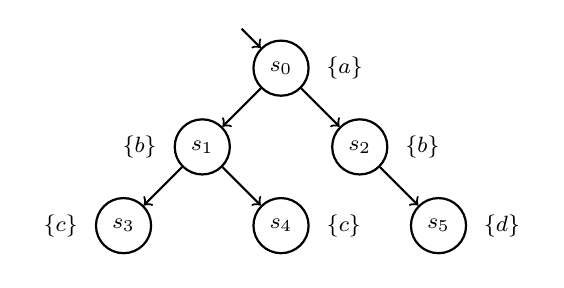
\begin{tikzpicture}[->,scale=1,label distance=0mm]
	\tikzstyle{every node}=[draw,shape=circle,minimum size=7mm,font=\footnotesize];
    \tikzstyle{every path}=[draw,thick];
    
    \node at (0, 0)  (s0) [label=right:${ \{a\} }$] {$s_0$};
    \node at (-1, -1) (s1) [label=left:${ \{b\} }$] {$s_1$};
    \node at (1, -1)  (s2) [label=right:${ \{b\} }$] {$s_2$};
    \node at (-2, -2)  (s3) [label=left:${ \{c\} }$] {$s_3$};
    \node at (0, -2)  (s4) [label=right:${ \{c\} }$] {$s_4$};
    \node at (2, -2)  (s5) [label=right:${ \{d\} }$] {$s_5$};

    \draw (-0.5, 0.5) to (s0);
    \draw (s0) to (s1);
    \draw (s0) to (s2);
	\draw (s1) to (s3);
	\draw (s1) to (s4);
    \draw (s2) to (s5);
\end{tikzpicture}
\end{center}

\begin{eqnarray*}
H_{0} &=&\{(s_{0},s_{0})\} \\
H_{1} &=&\{(s_{0},s_{0}),(s_{1},s_{1})\} \\
H_{2} &=&\{(s_{0},s_{0}),(s_{1},s_{1}),(s_{2},s_{2})\} \\
H_{3} &=&\{(s_{0},s_{0}),(s_{1},s_{1}),(s_{2},s_{2}),(s_{3},s_{3})\} \\
H_{4}
&=&\{(s_{0},s_{0}),(s_{1},s_{1}),(s_{2},s_{2}),(s_{3},s_{3}),(s_{4},s_{4})\}
\\
H_{5}
&=&%
\{(s_{0},s_{0}),(s_{1},s_{1}),(s_{2},s_{2}),(s_{3},s_{3}),(s_{4},s_{4}),(s_{5},s_{5})\}
\\
H_{6} &=&H_{5}
\end{eqnarray*}

\bigskip

\newpage

\end{document}

